‫\فصل{نمونه اولیه واسط کاربری}
‫\قسمت{صفحه لاگین}
‫بعد از اجرای برنامه این صفحه بالا می‌آید و از کاربر می‌خواهد که شماره تلفن یا ایمیل خود را به همراه رمز عبور وارد کند و در صورتی که اکانتی نداشته باشد باید به صفحه رجیستر برود.
‫\\
‫\شروع{شکل}[ht]
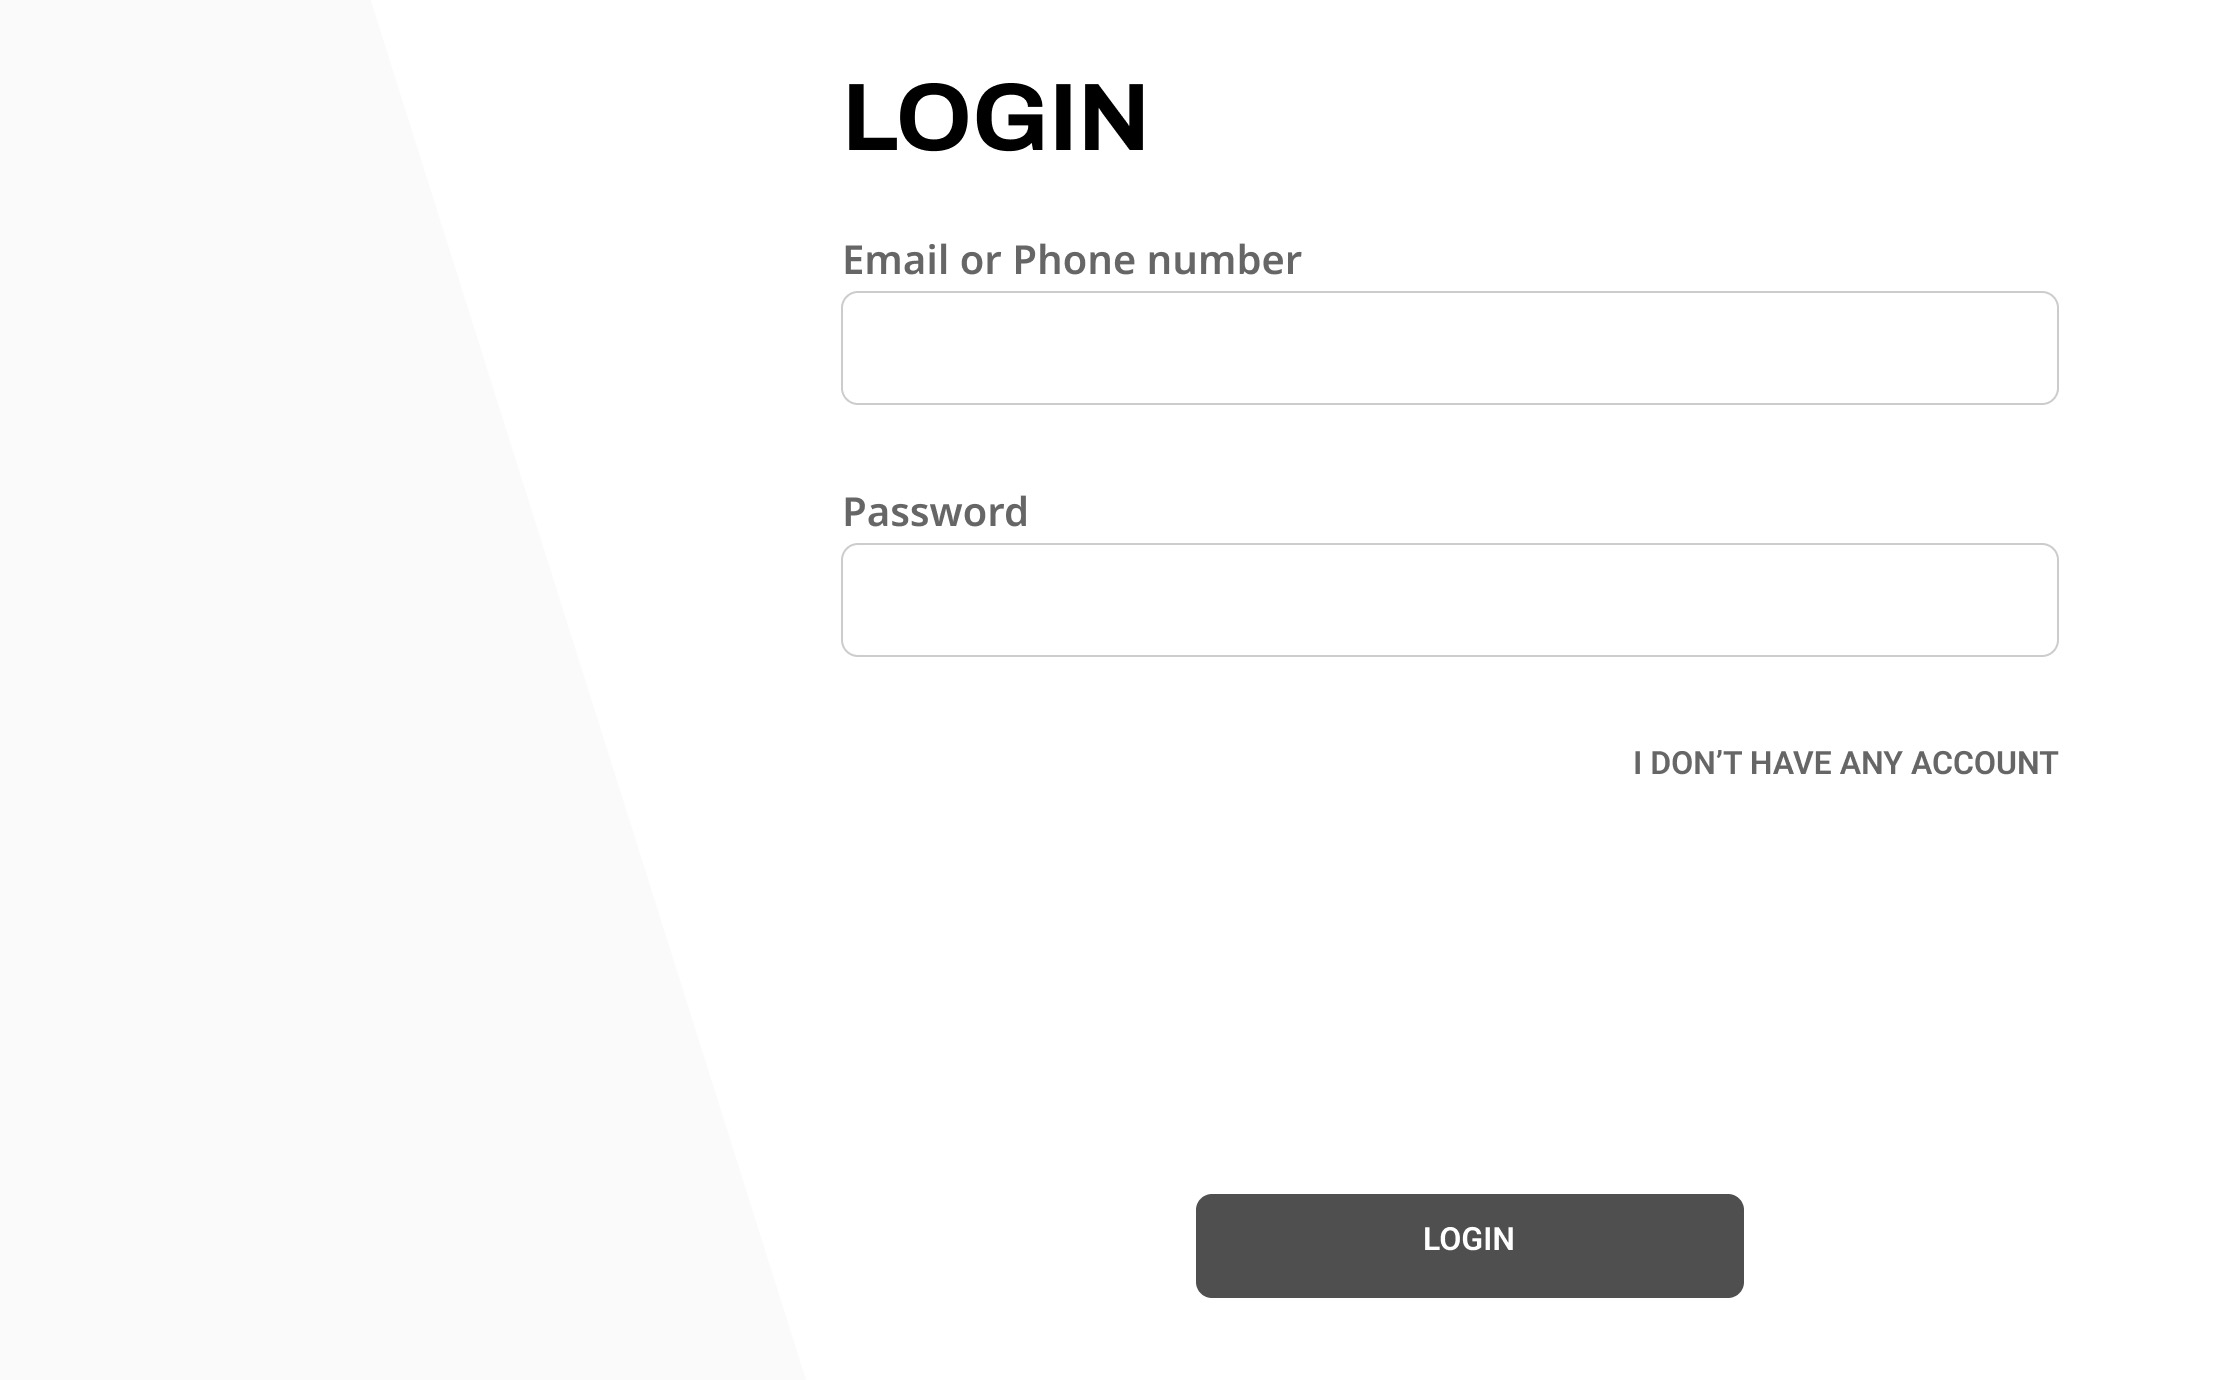
\includegraphics[scale=0.2]{figs/login_page.jpeg}
‫\شرح{صفحه لاگین}
‫\برچسب{شکل:صفحه لاگین}
‫\پایان{شکل}
‫
‫
‫\قسمت{صفحه رجیستر}
‫بعد از اجرای برنامه در صورتی که اکانتی کاربر نداشته باشد، از صفحه لاگین به این صفحه می‌آید و اکانت می‌سازد.
\\
‫\شروع{شکل}[ht]
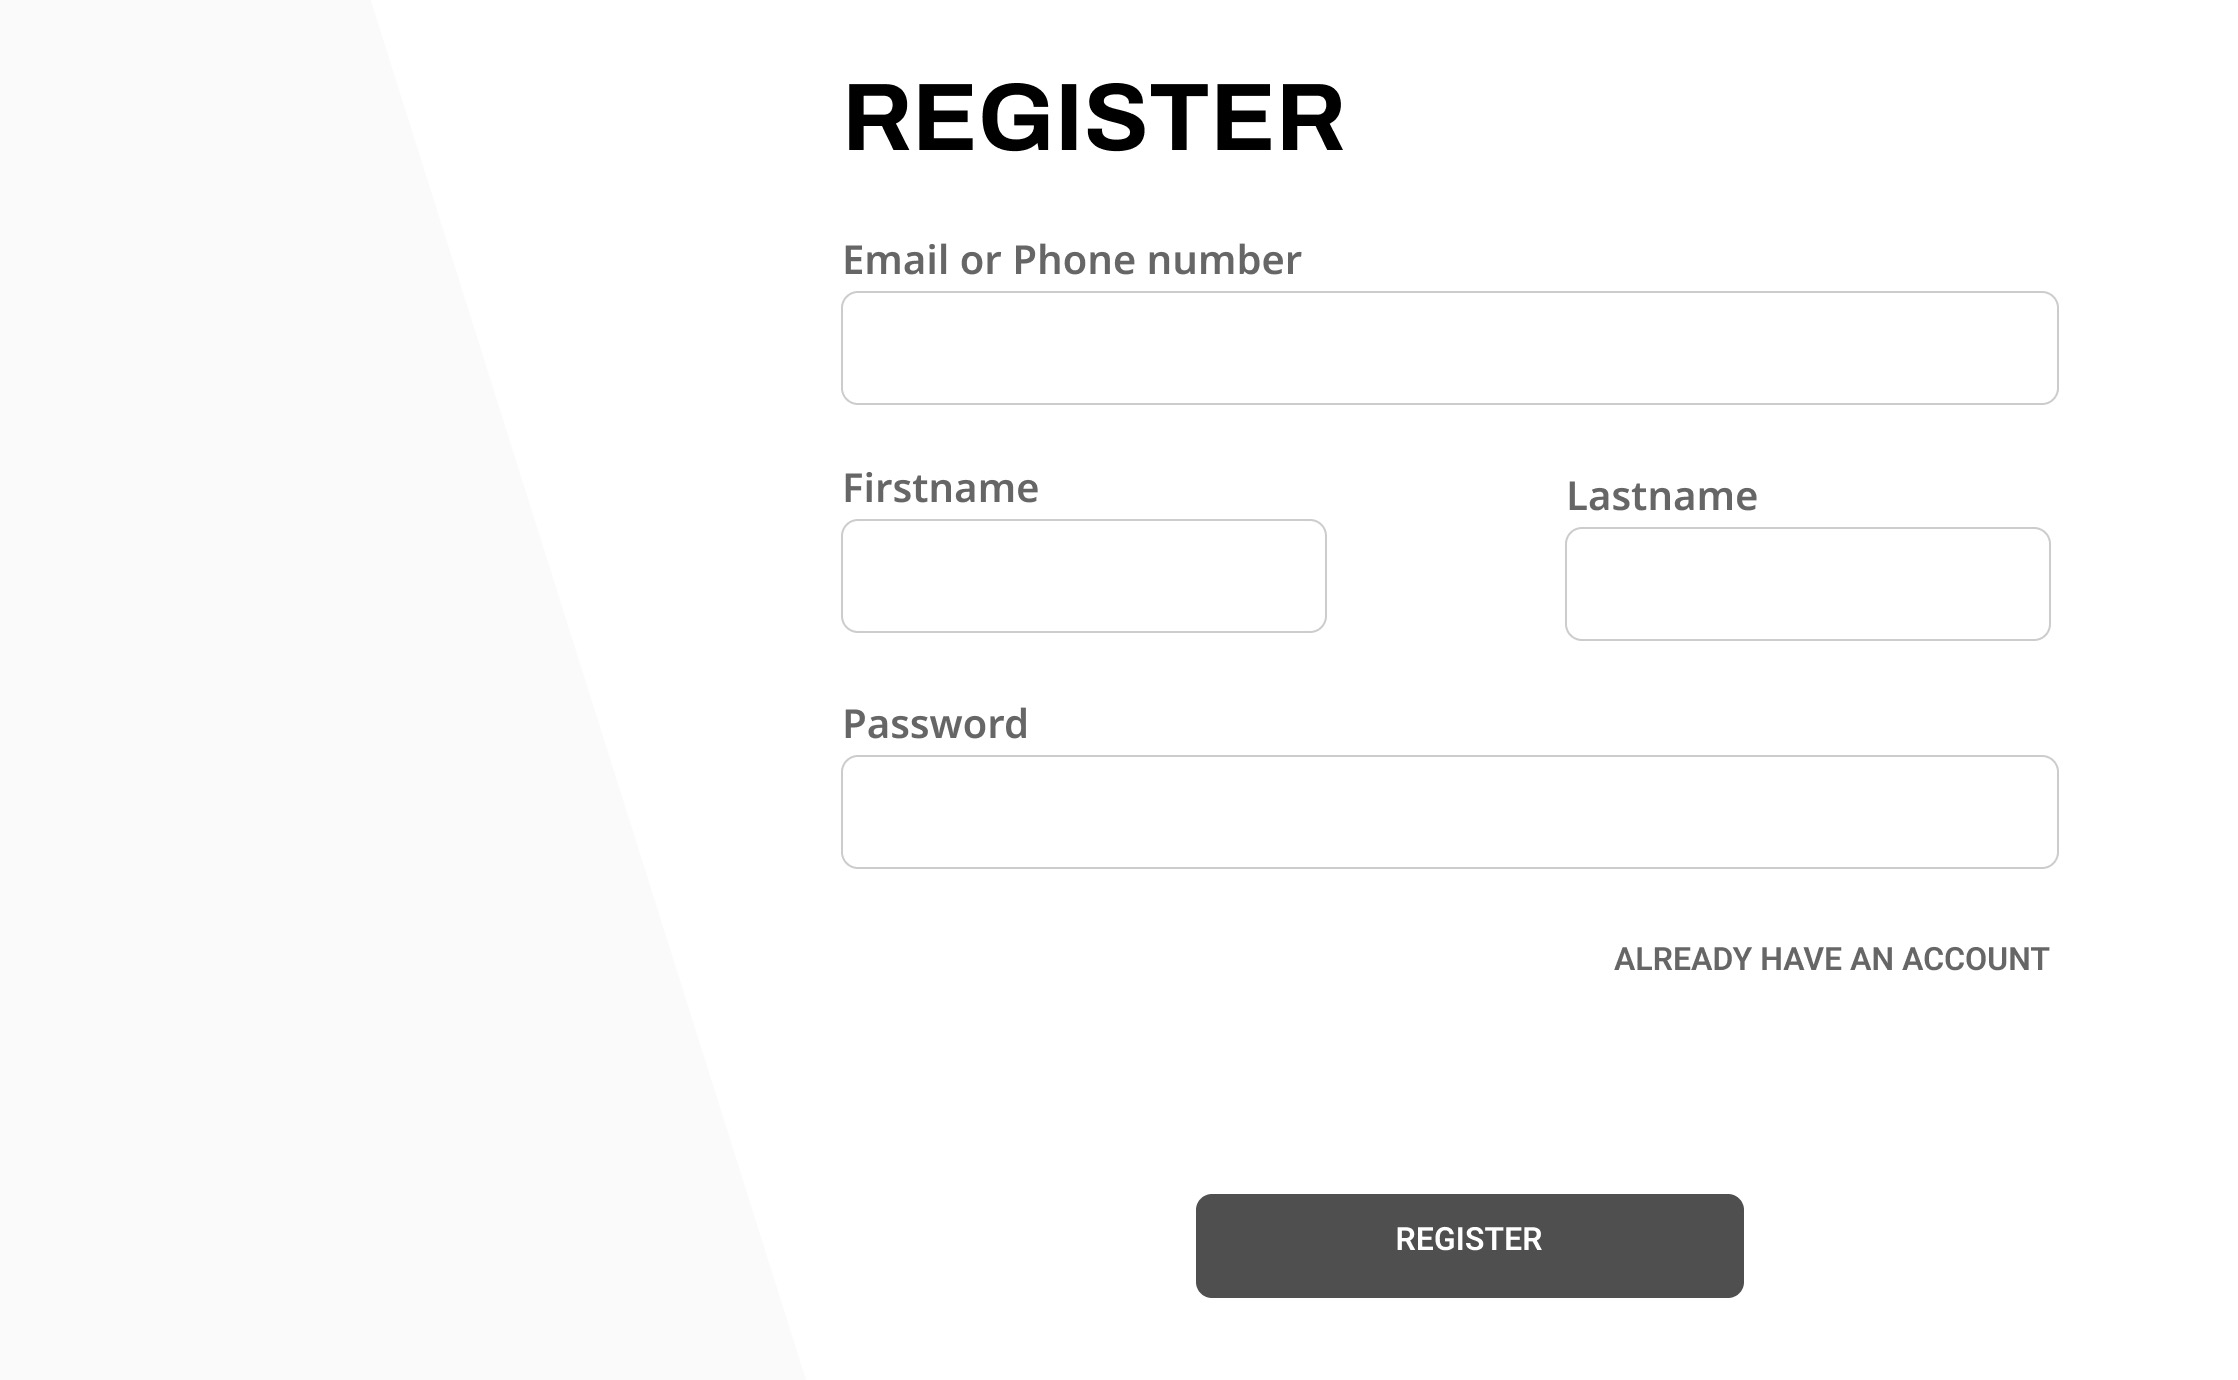
\includegraphics[scale=0.2]{figs/register_page.jpeg}
‫\شرح{صفحه رجیستر}
‫\برچسب{شکل:صفحه رجیستر}
‫\پایان{شکل}
\clearpage


‫\قسمت{صفحه کانال برای کاربر}
‫بعد از ورود برای کاربران لیستی از کانال‌هایی که عضو آن هستند می‌آید و در صورتی که مشاهده محتوا کانال از سوی مدیر کانال رایگان تعریف شده باشد، می‌تواند محتوا را به طور کامل ببیند. در صورتی که برای دیدن محتوا‌ها حق عضویت تعریف شده باشد تنها عنوان و بخشی از متن را می‌بیند و در صورتی که بر روی مشاهده بیشتر کلیک کنند، صفحه‌ای می‌آید که توضیحاتی در رابطه با حق عضویت بیان می‌کند و در صورتی که گزینه‌ای را انتخاب که بخواهد حق عضویت را خریداری کند، در صورت داشتن مقدار پول در حساب خود از آن کم می‌شود یا به صفحه پرداخت هدایت می‌شود.
‫\\
‫\شروع{شکل}[ht]
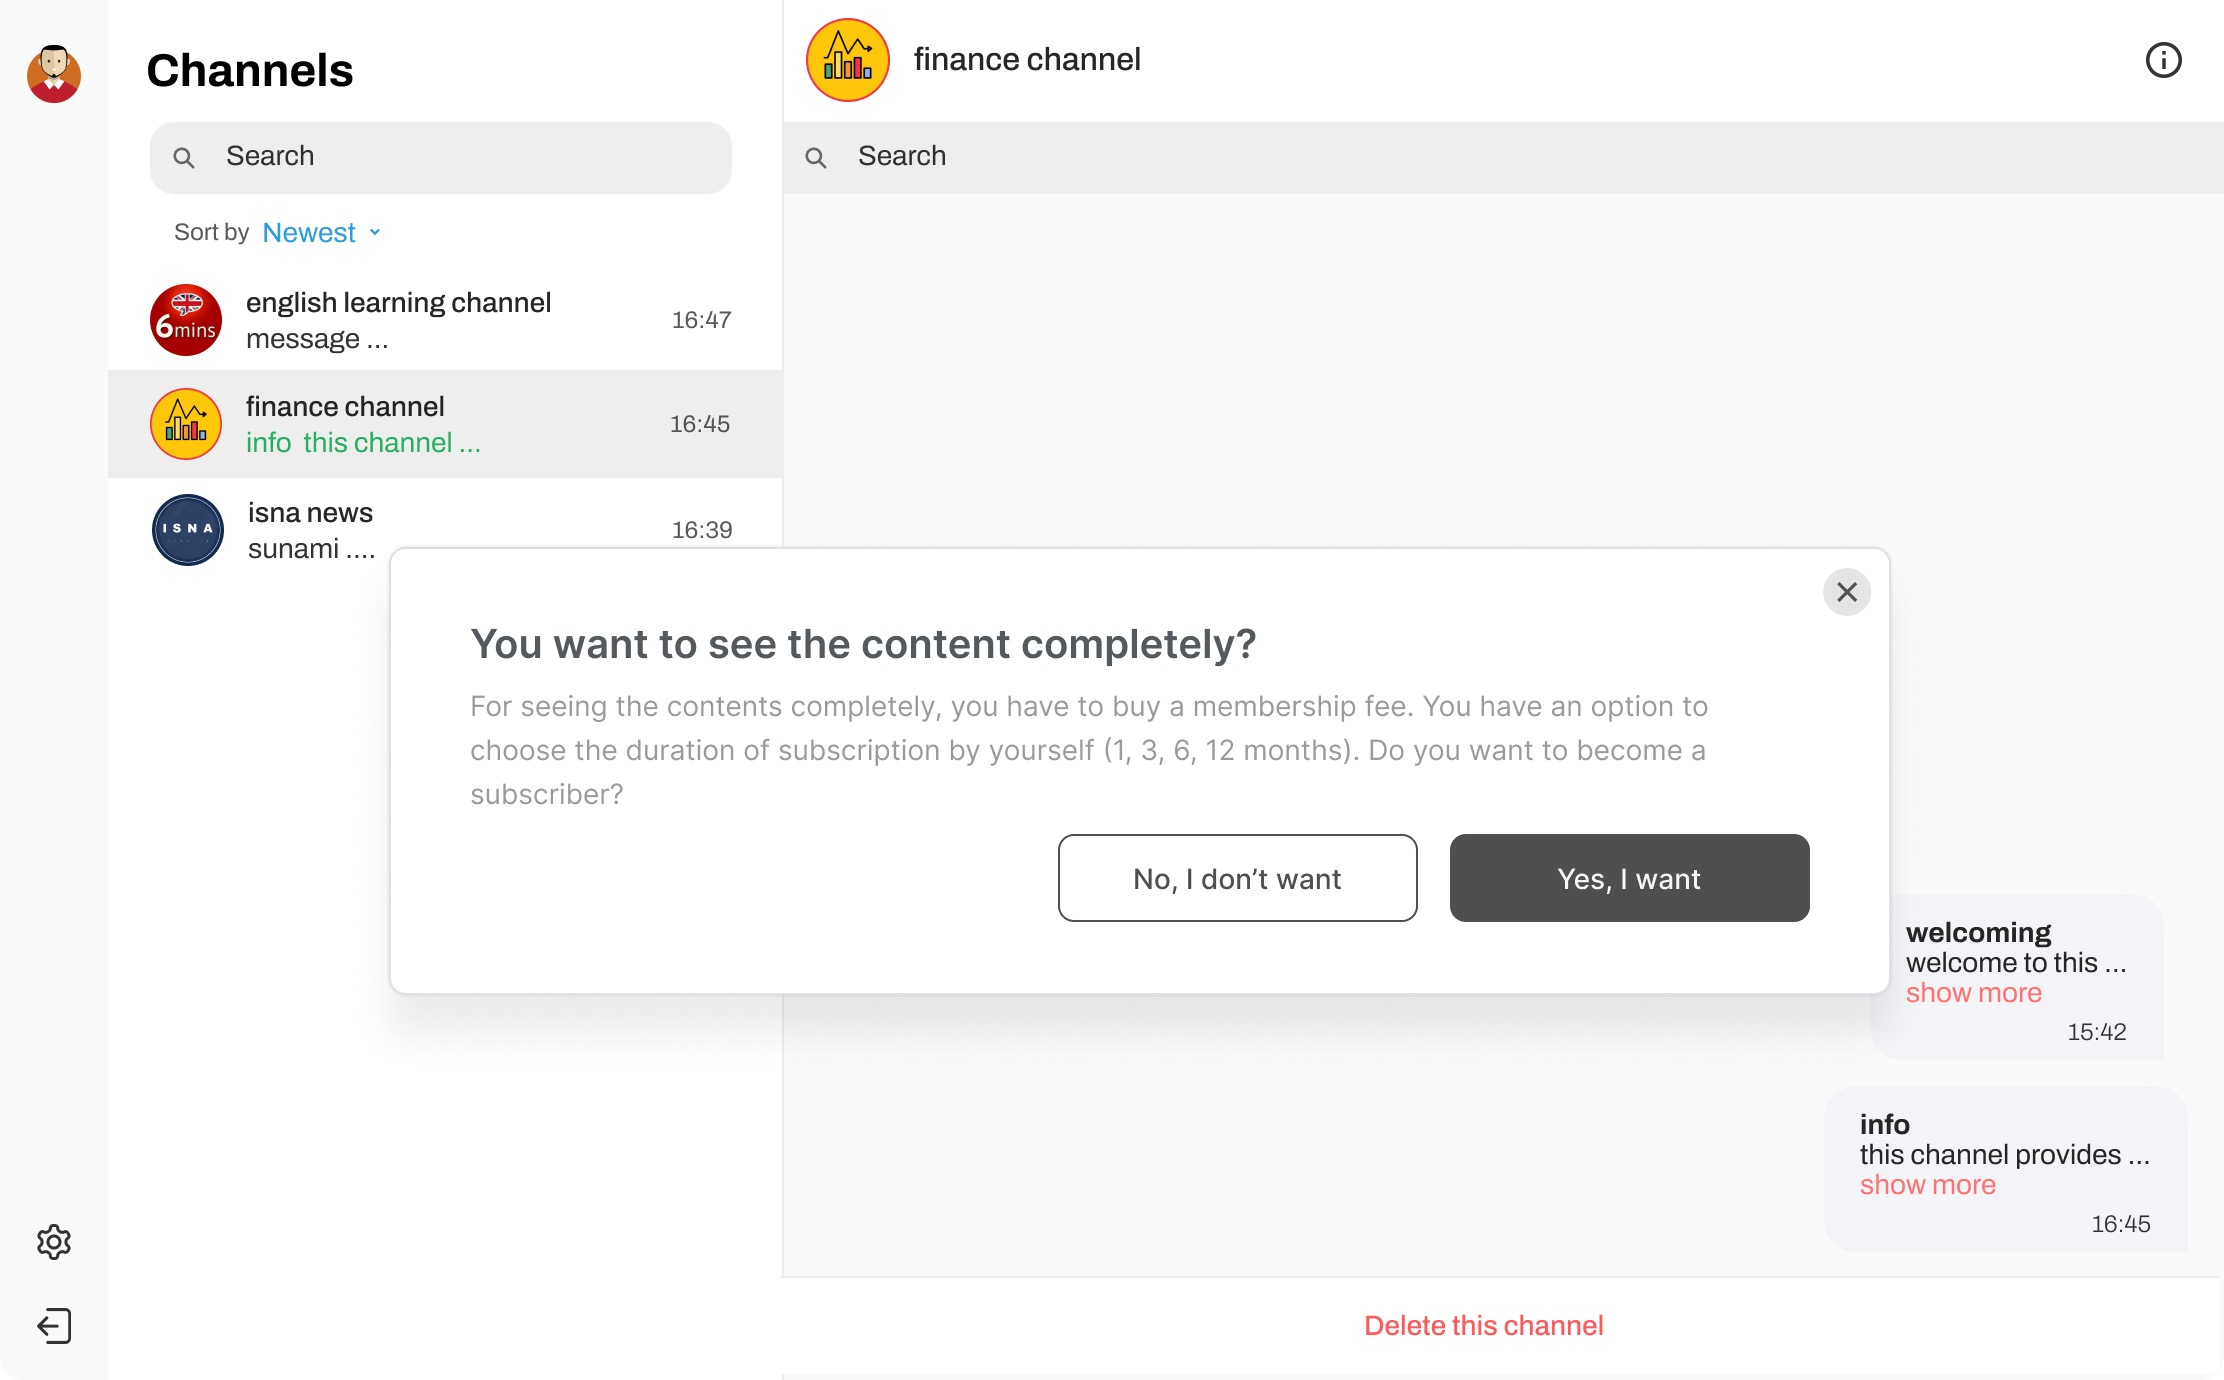
\includegraphics[scale=0.2]{figs/user_channel_page.jpeg}
‫\شرح{صفحه کانال برای کاربر}
‫\برچسب{شکل:صفحه کانال برای کاربر}
‫\پایان{شکل}
‫\FloatBarrier

\clearpage
‫
‫\قسمت{صفحه کانال برای مدیر یا صاحب کانال}
‫بعد از ورود برای مدیر لیستی از کانال‌هایی که مدیر آن هستند می‌آید و می‌توانند در آن محتوا‌های نظیر متن، تصویر، ویدیو و صدا در آن قرار دهد که کاربران عضو آن بتواند از آن محتوا استفاده کنند. همچنین قابلیت ادیت و پاک کردن پیام‌ها را نیز دارد.
‫\\
‫‫\شروع{شکل}[ht]
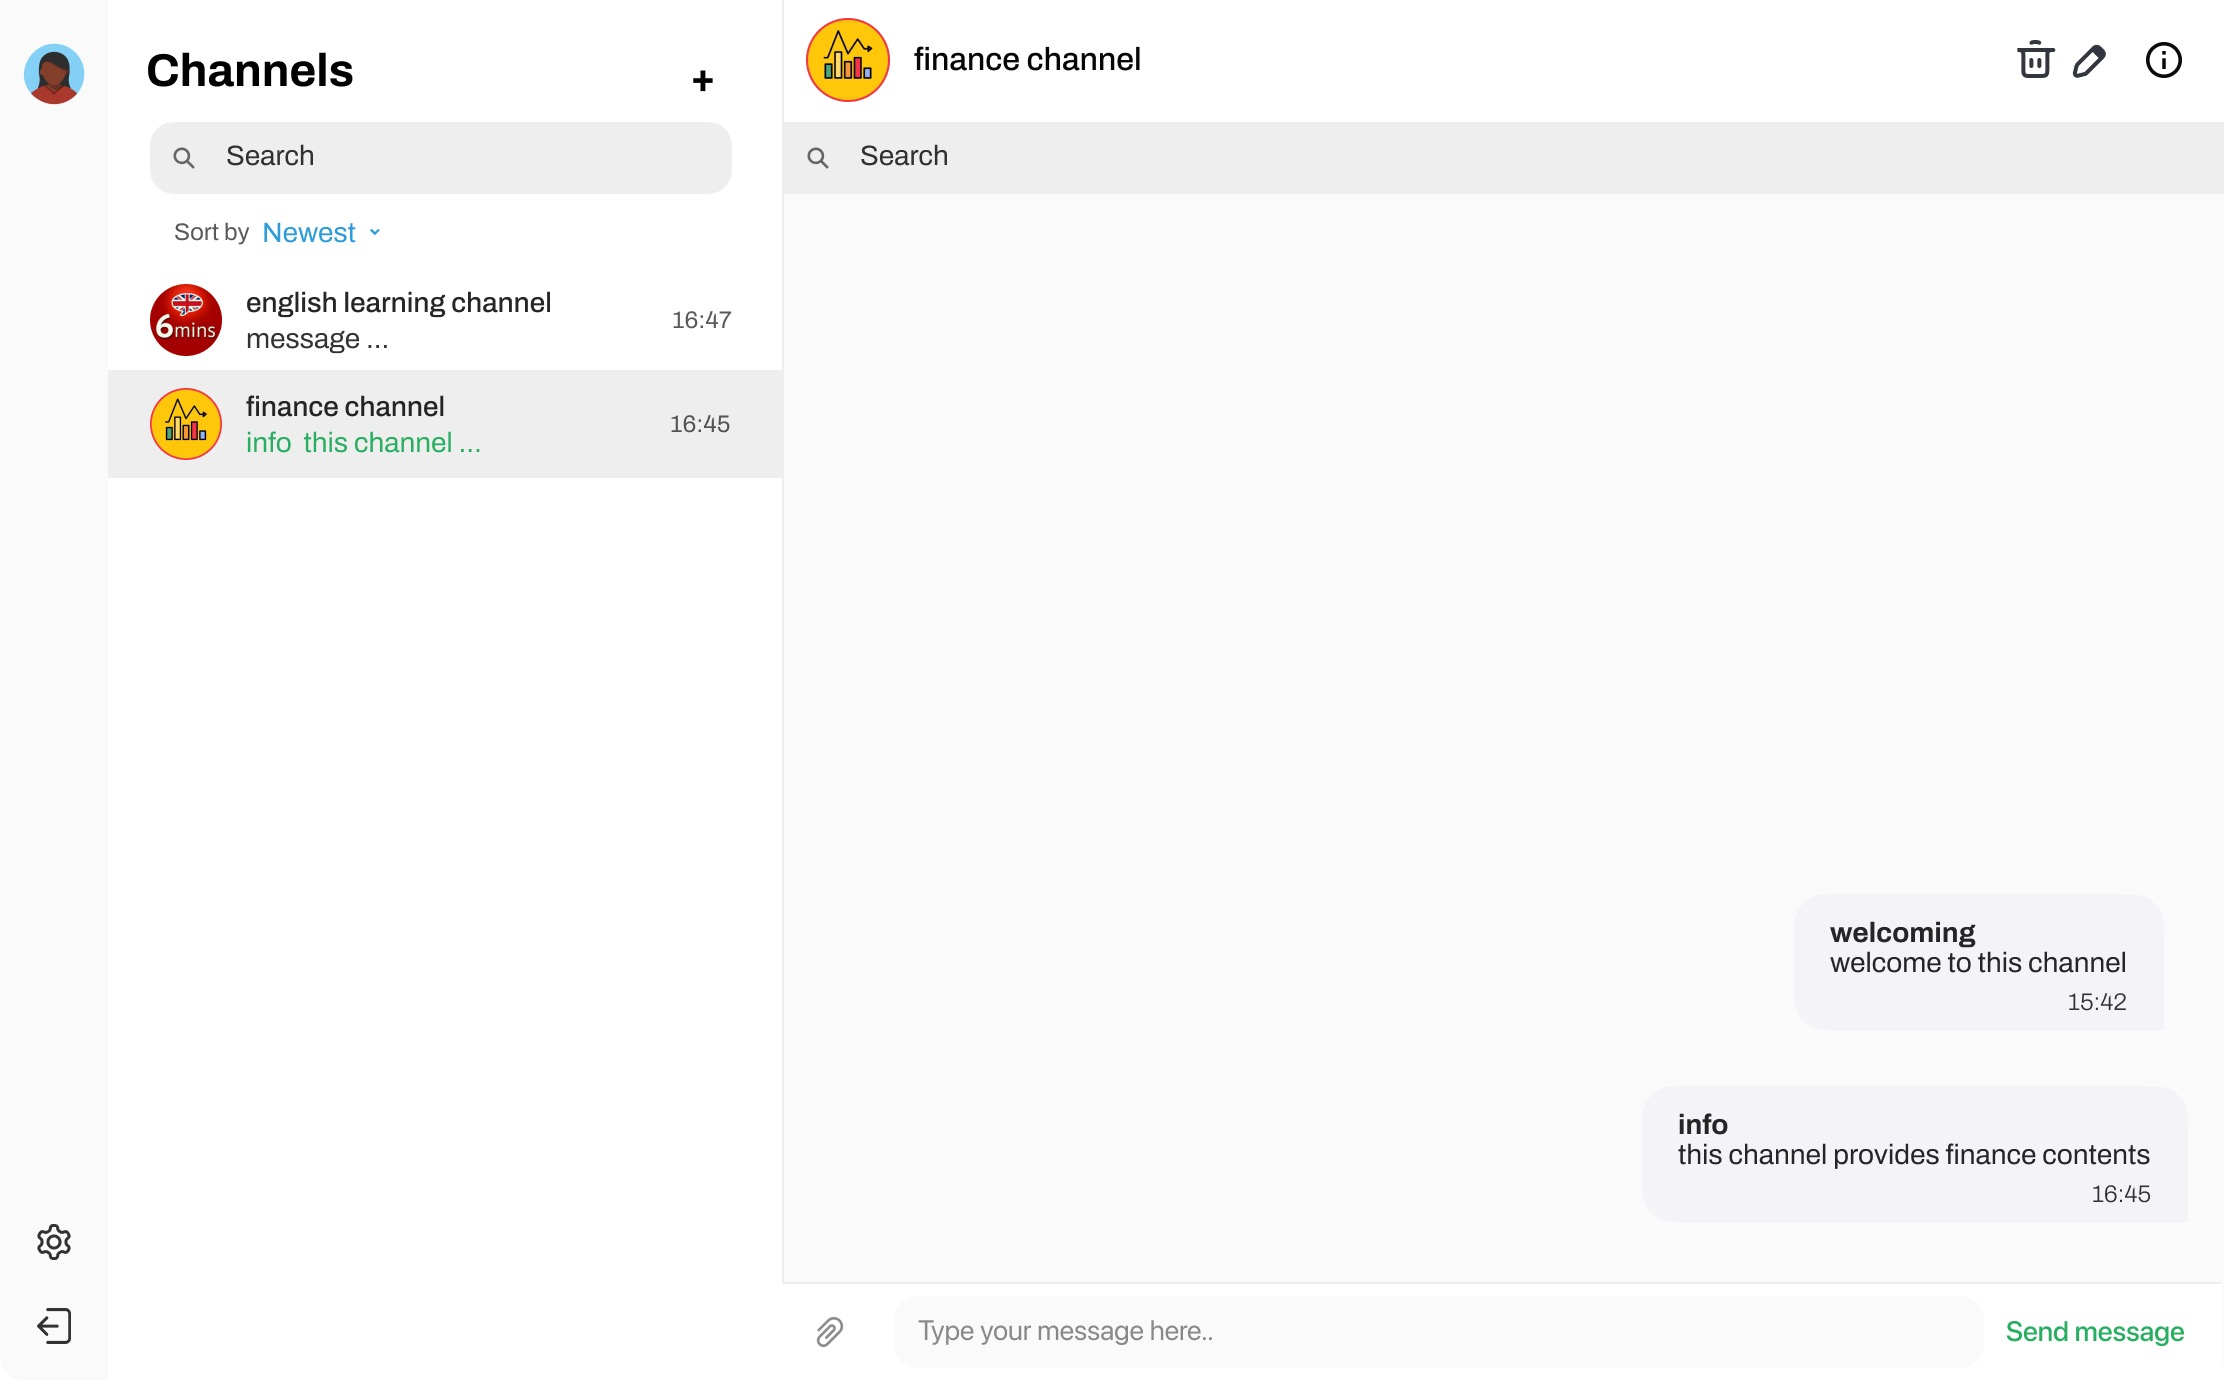
\includegraphics[scale=0.2]{figs/admin_channel_page.jpeg}
‫\شرح{صفحه کانال برای مدیر یا صاحب کانال}
‫\برچسب{شکل:صفحه کانال برای مدیر یا صاحب کانال}
‫\پایان{شکل}
‫ \FloatBarrier
\clearpage

‫
‫\قسمت{صفحه اطلاعات کانال برای صاحب کانال}
‫این صفحه شامل اعضای کانال است که مدیر می‌تواند کاربرانی را که حق عضویت ندارند، حذف کند. همچنین می‌تواند مدیر کانال، میزان درصد سود برای مدیر و هزینه‌های حق عضویت را تغییر دهد یا آن را در صورتی که رایگان می‌باشد به حالتی که نیاز به حق عضویت دارد تغییر بدهد.
‫\\
‫\شروع{شکل}[ht]
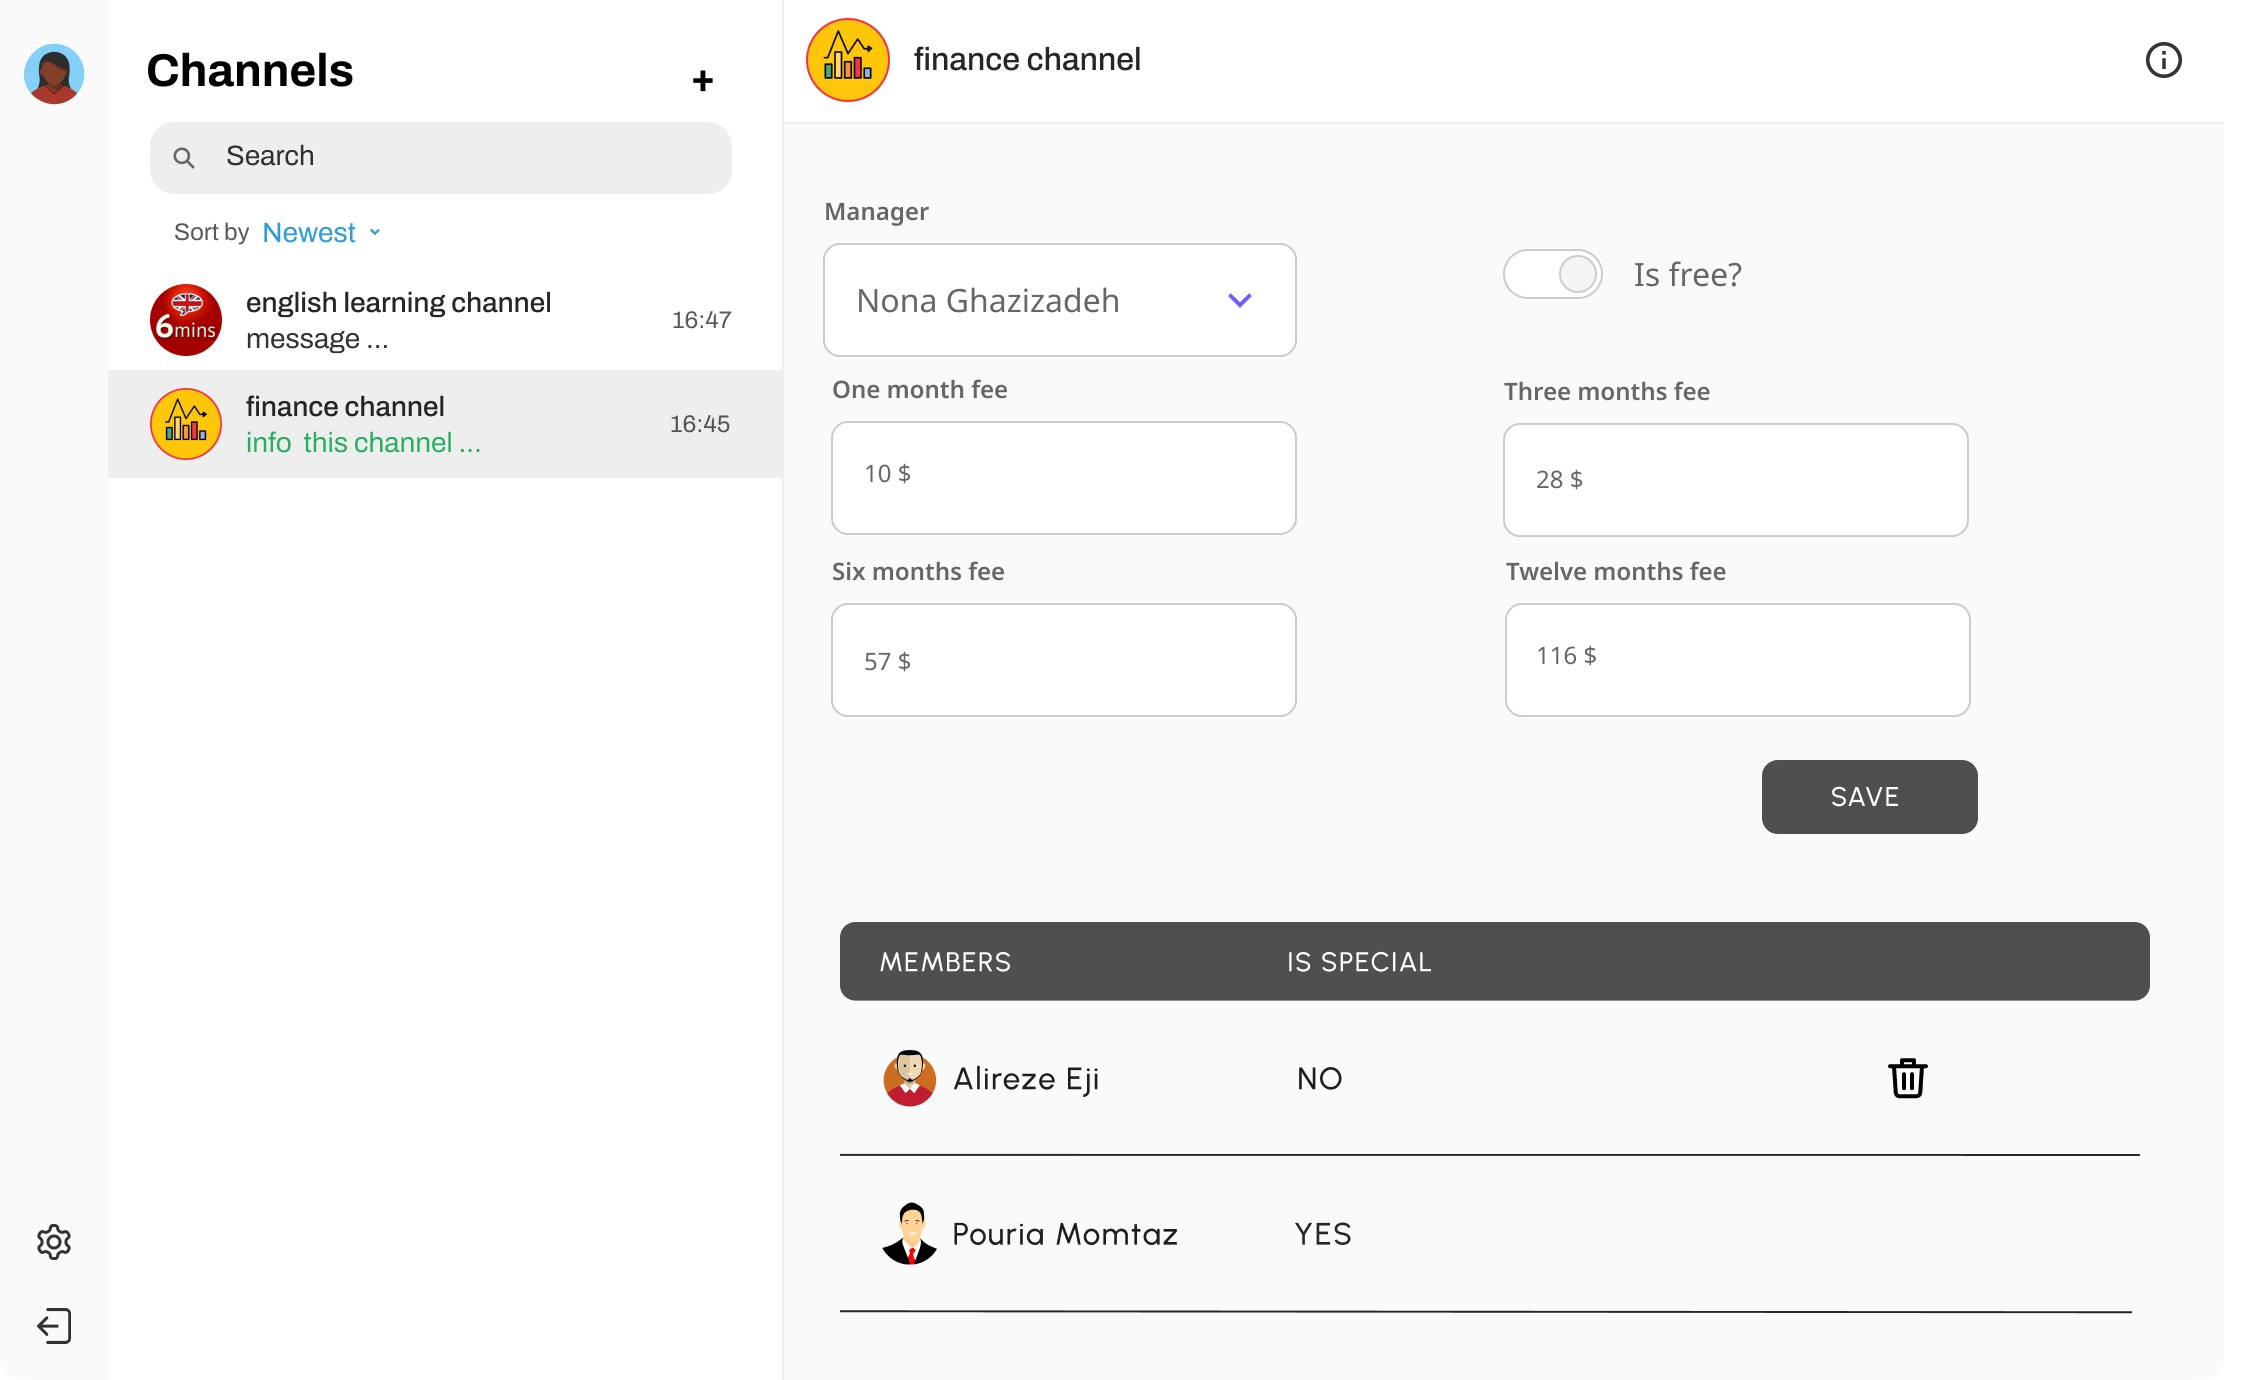
\includegraphics[scale=0.2]{figs/info_admin_channel_page.jpeg}
‫\شرح{صفحه اطلاعات کانال برای صاحب کانال}
‫\برچسب{شکل:صفحه اطلاعات کانال برای صاحب کانال}
‫\پایان{شکل}
‫\FloatBarrier
\clearpage

‫
‫\قسمت{صفحه اطلاعات کانال برای کاربران}
‫این صفحه شامل اطلاعات حق عضویت برای کاربران است در صورتی که کاربر بخواهند محتوا کانال را به صورت کامل ببیند باید یکی از حق عضویت‌ها را خریداری کند.
‫\\
‫\شروع{شکل}[ht]
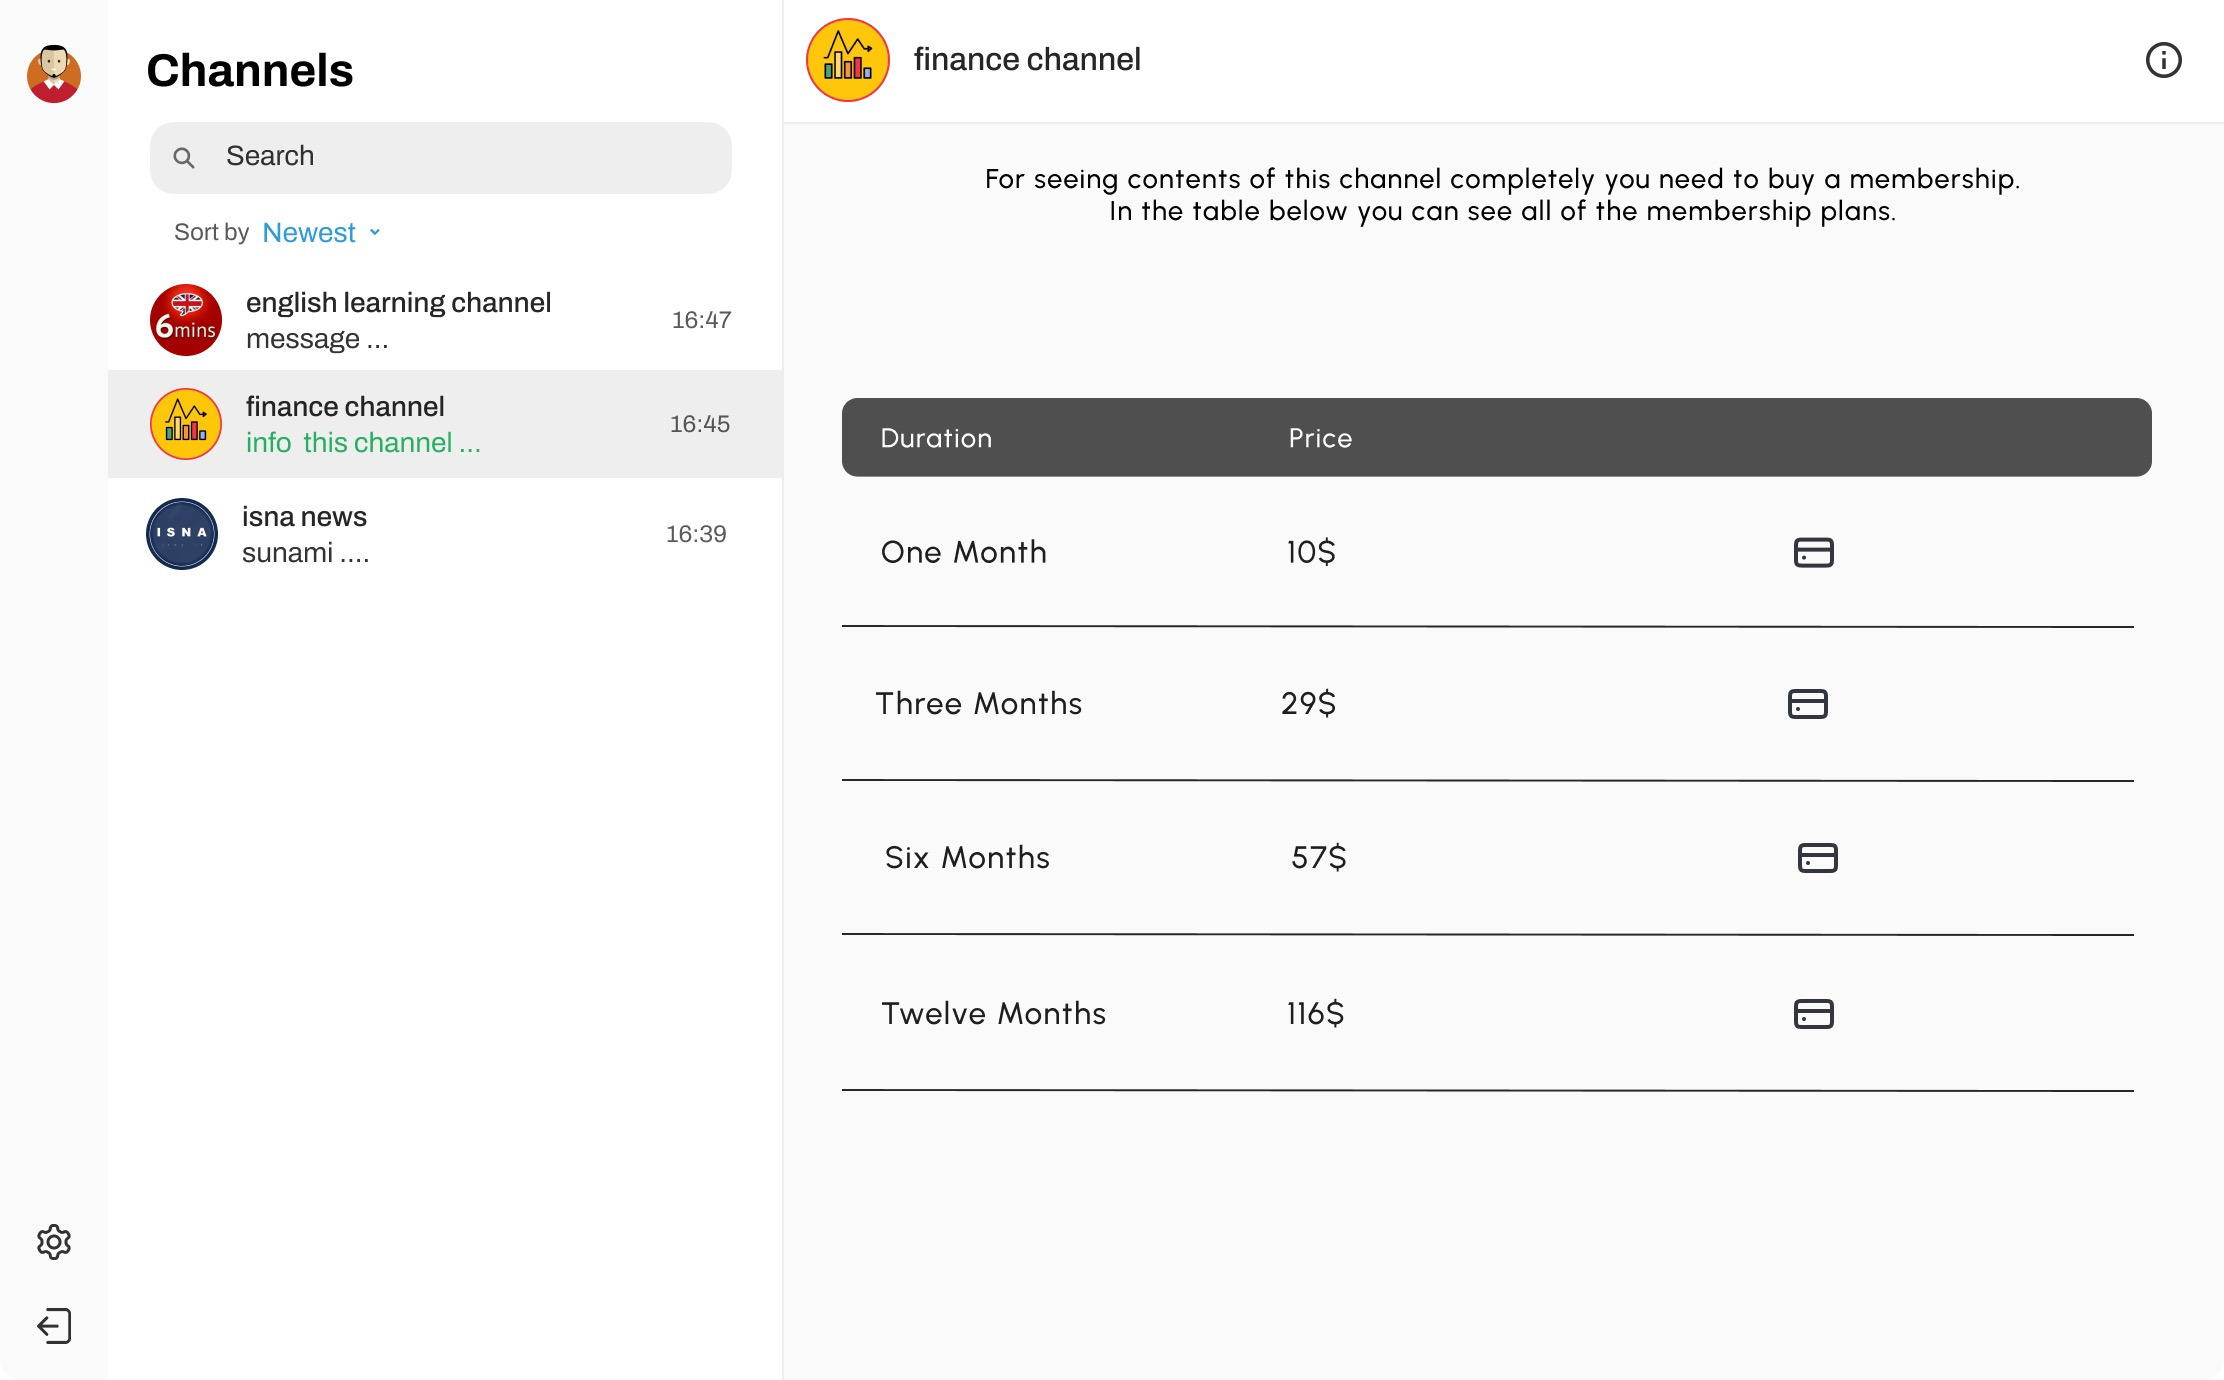
\includegraphics[scale=0.2]{figs/info_user_channel_page.jpeg}
‫\شرح{صفحه اطلاعات کانال برای کاربران}
‫\برچسب{شکل:صفحه اطلاعات کانال برای کاربران}
‫\پایان{شکل}
‫‫ \FloatBarrier
‫\clearpage
‫
‫\قسمت{صفحه اطلاعات مالی کاربر}
‫این صفحه شامل اطلاعات درآمدی از کانال‌هایی که مدیر یا صاحب آن‌ها هستند را نشان می‌دهد.
‫\\
‫\شروع{شکل}[ht]
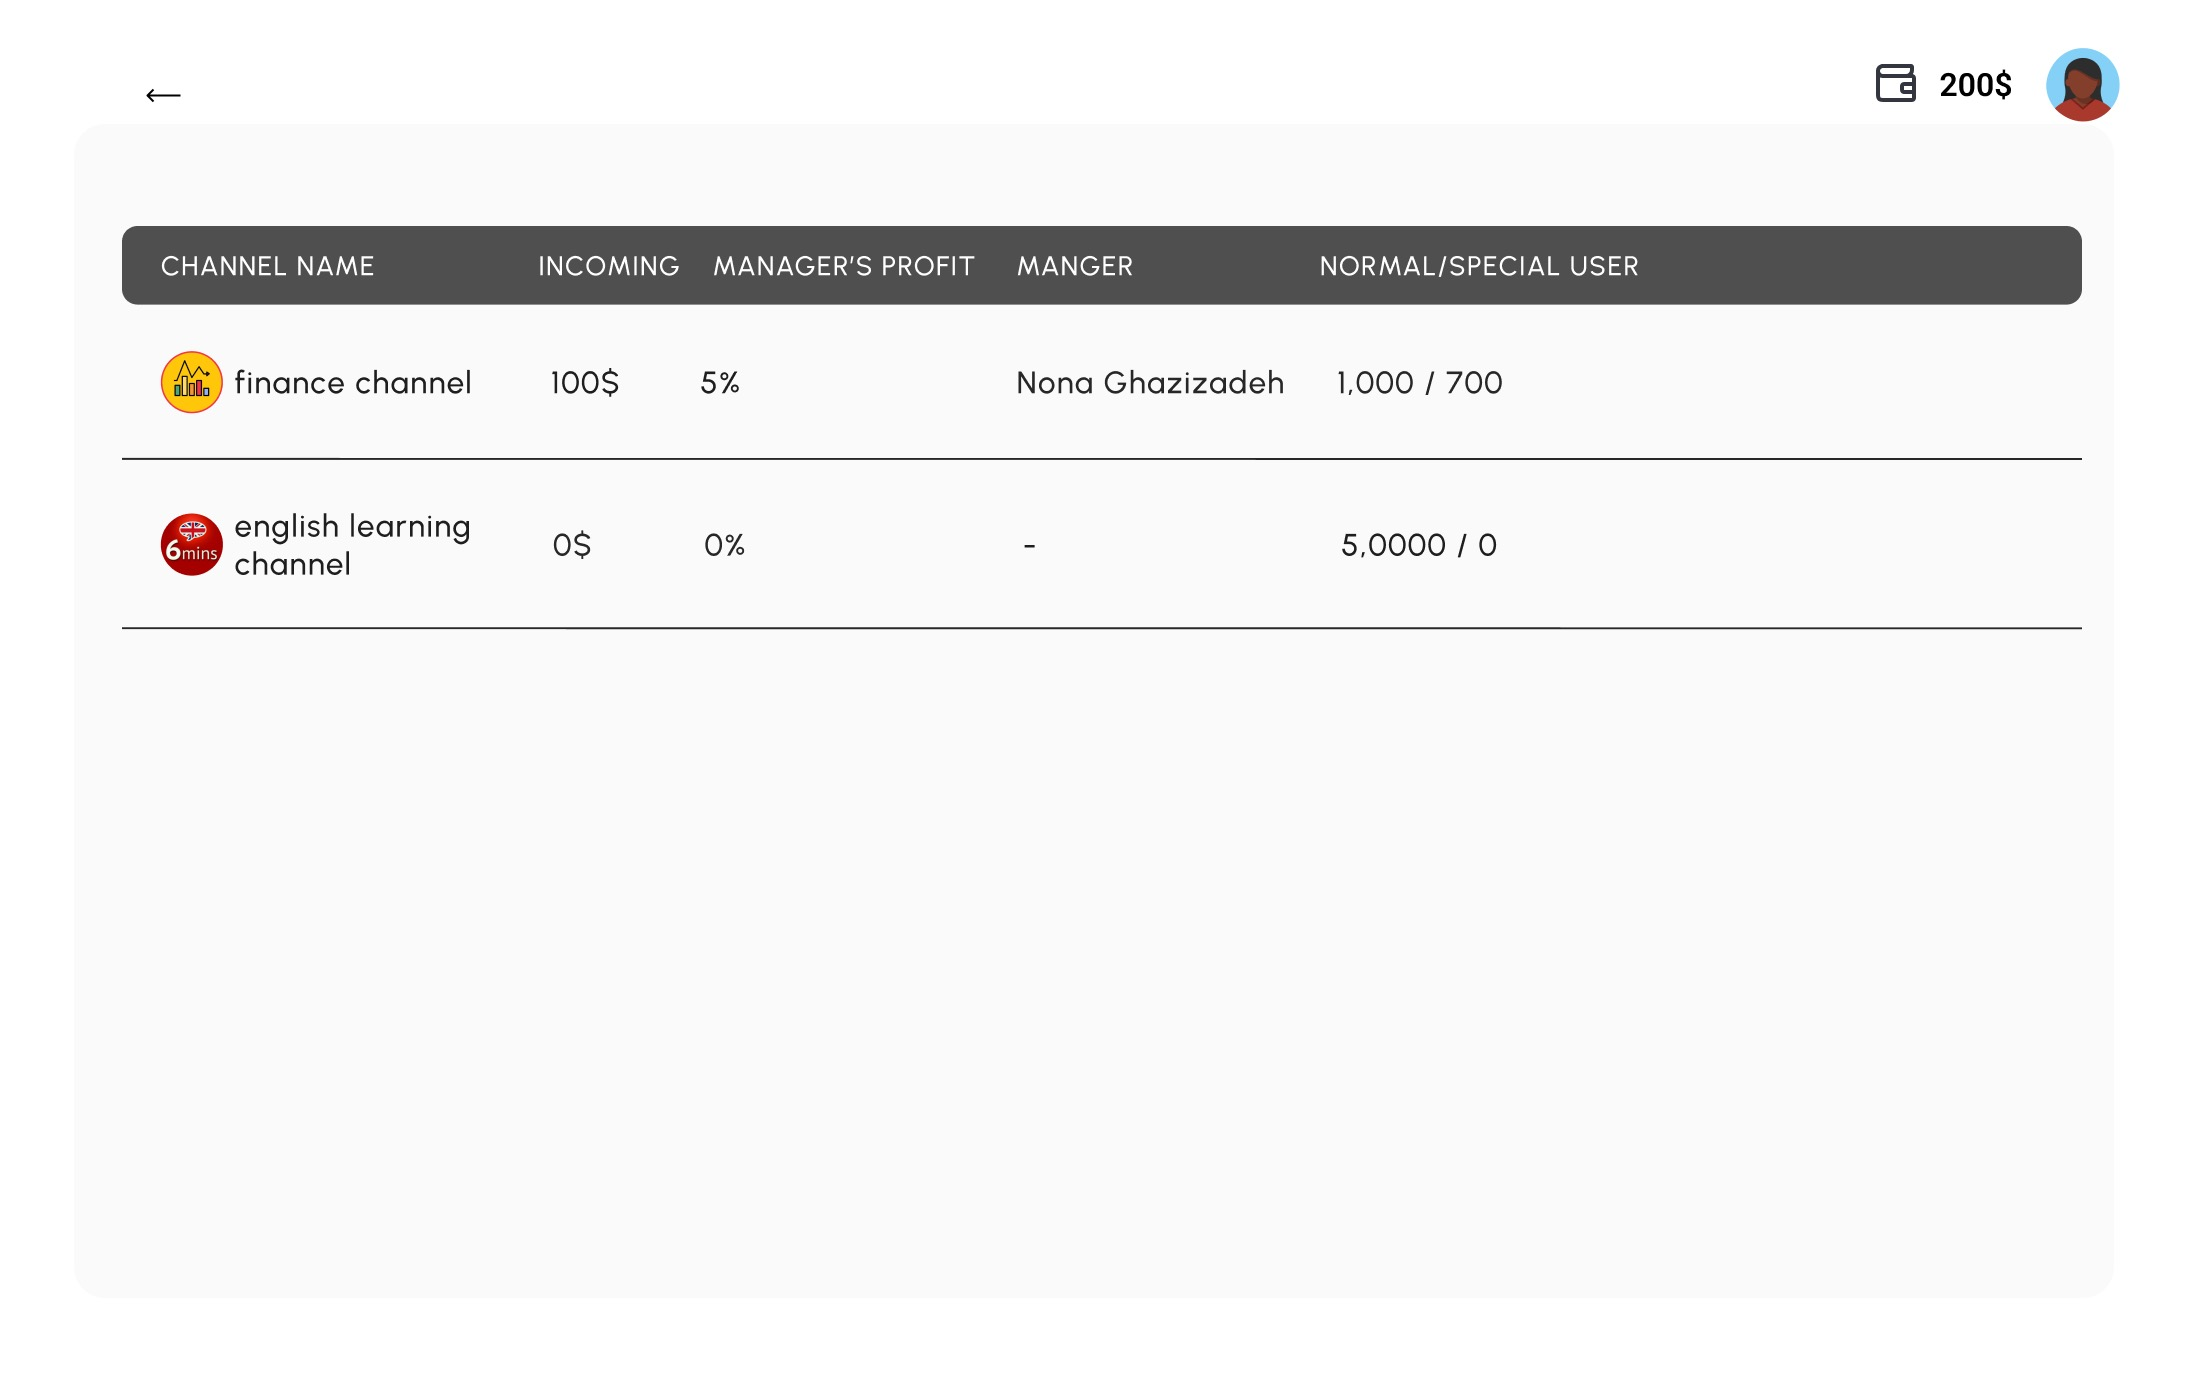
\includegraphics[scale=0.2]{figs/admin_page.jpeg}
‫\شرح{صفحه کاربری صاحب}
‫\برچسب{شکل:صفحه کاربری صاحب}
‫\پایان{شکل}
‫‫ \FloatBarrier
‫\clearpage
‫
‫\قسمت{صفحه کاربری کاربر}
‫این صفحه شامل اطلاعات کاربری است و می‌تواند نام و نام خانوادگی و رمز عبور را تغییر بدهد. همچنین میزان پولی را که در حسابش است نشان می‌دهد و می‌تواند کیف‌پول خود را شارژ کند.
‫\\
‫\شروع{شکل}[ht]
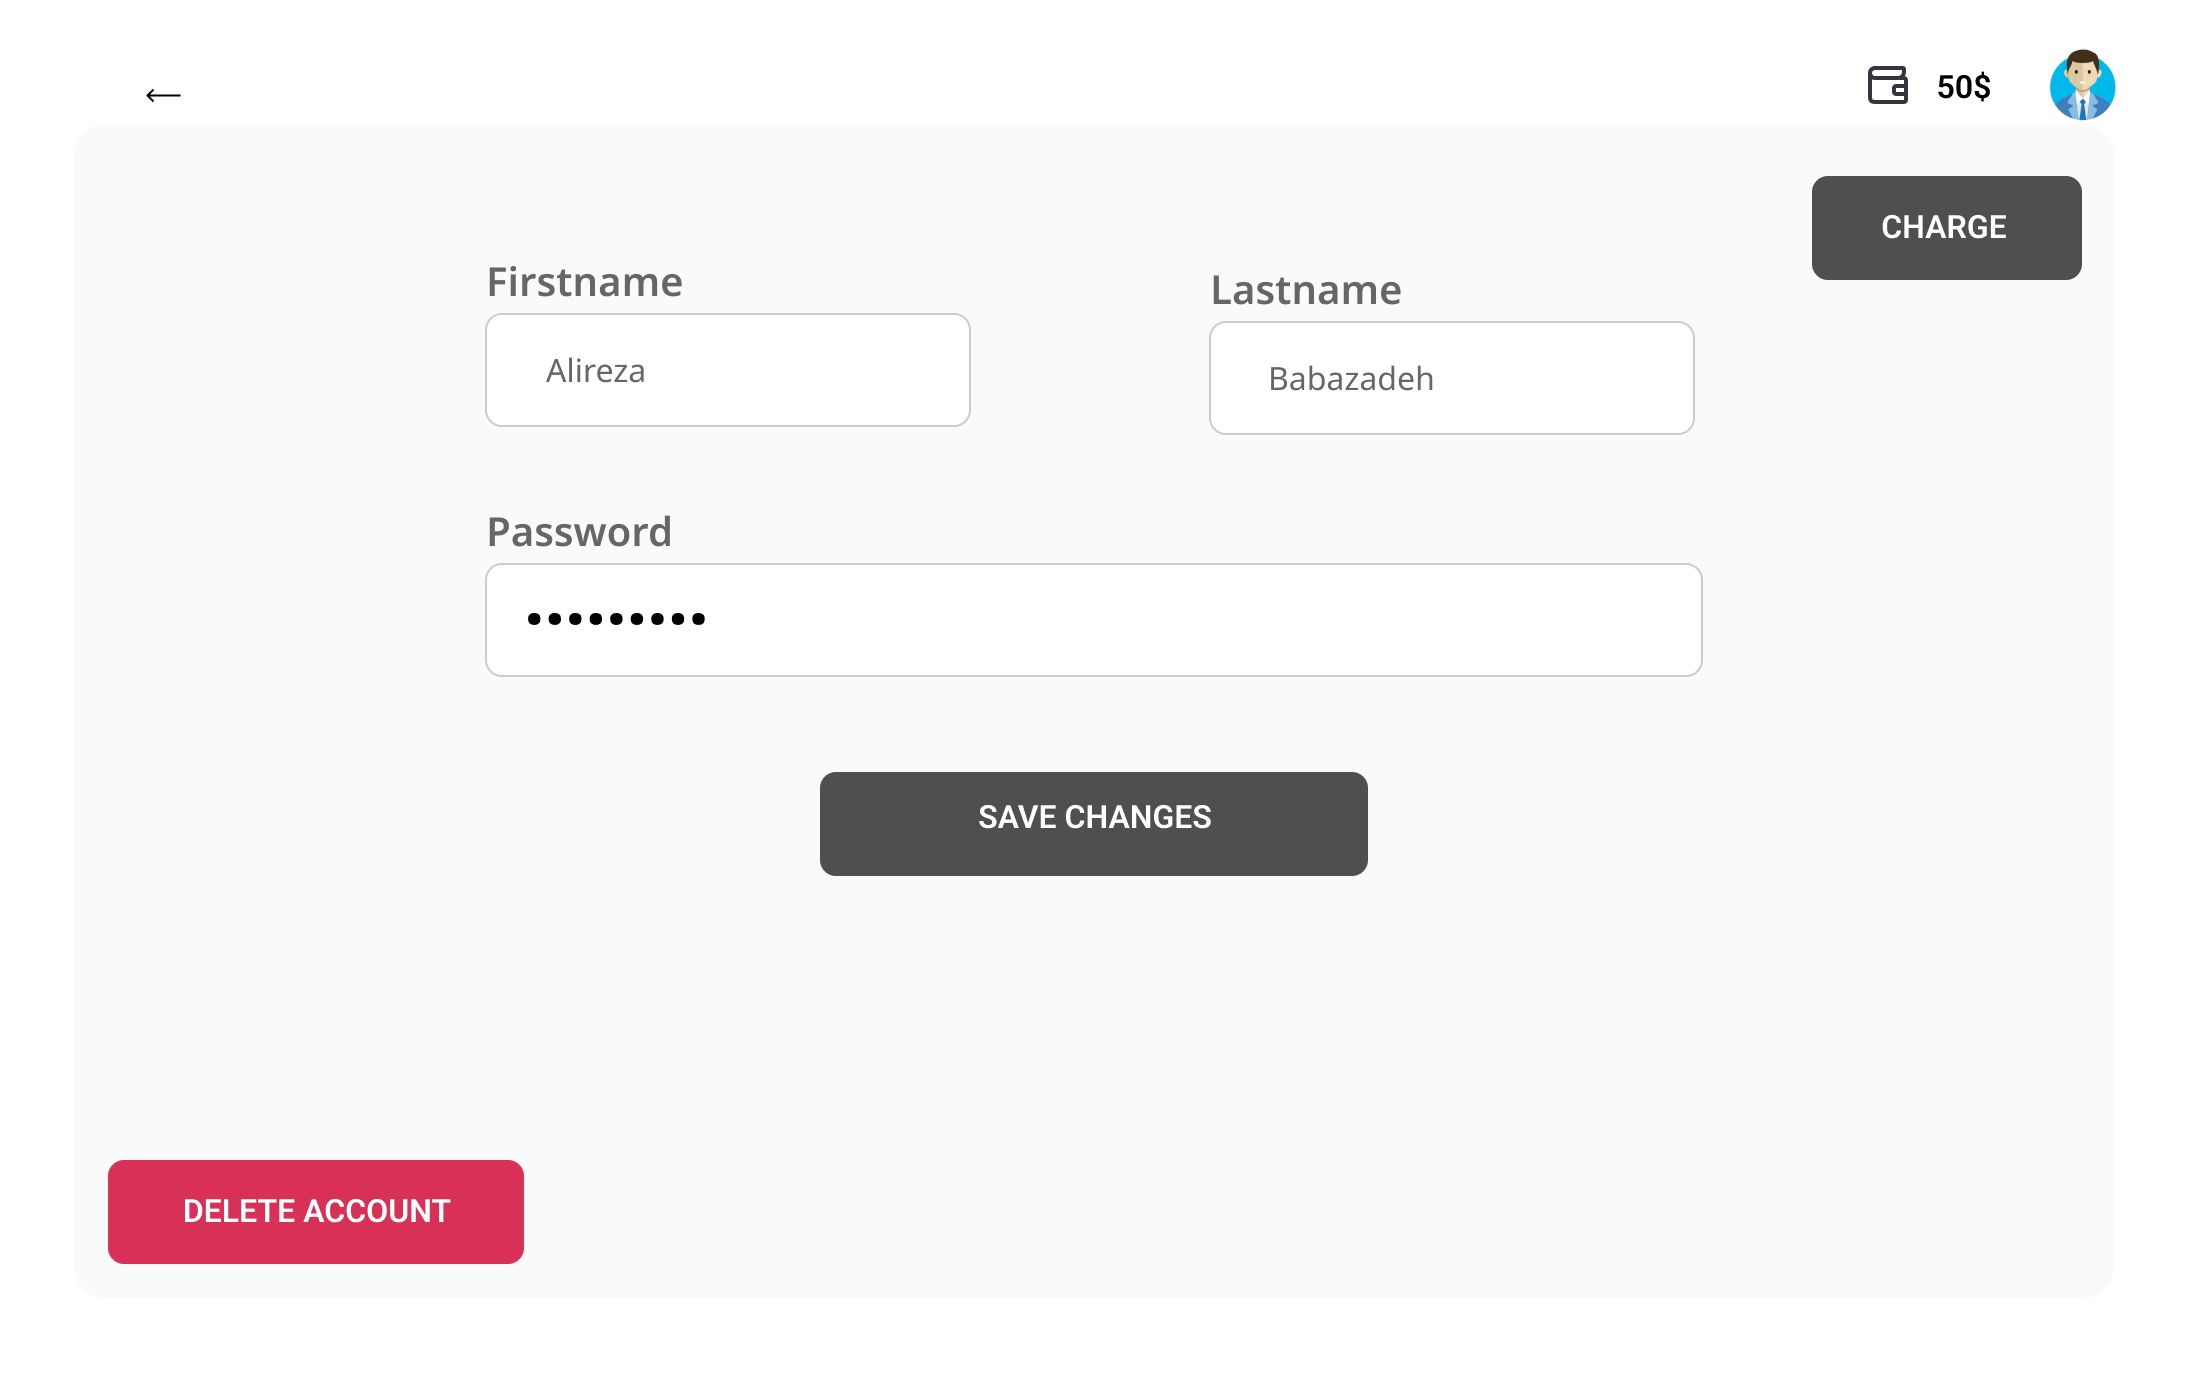
\includegraphics[scale=0.2]{figs/user_page.jpeg}
‫\شرح{صفحه کاربری کاربر}
‫\برچسب{شکل:صفحه کاربری کاربر}
‫\پایان{شکل}
‫‫ \FloatBarrier
‫\clearpage
‫
‫\قسمت{صفحه ساخت کانال}
‫این صفحه برای ایجاد کانال است و اطلاعات مرتبط را از صاحب آن می‌گیرد 
‫\\
‫\شروع{شکل}[ht]
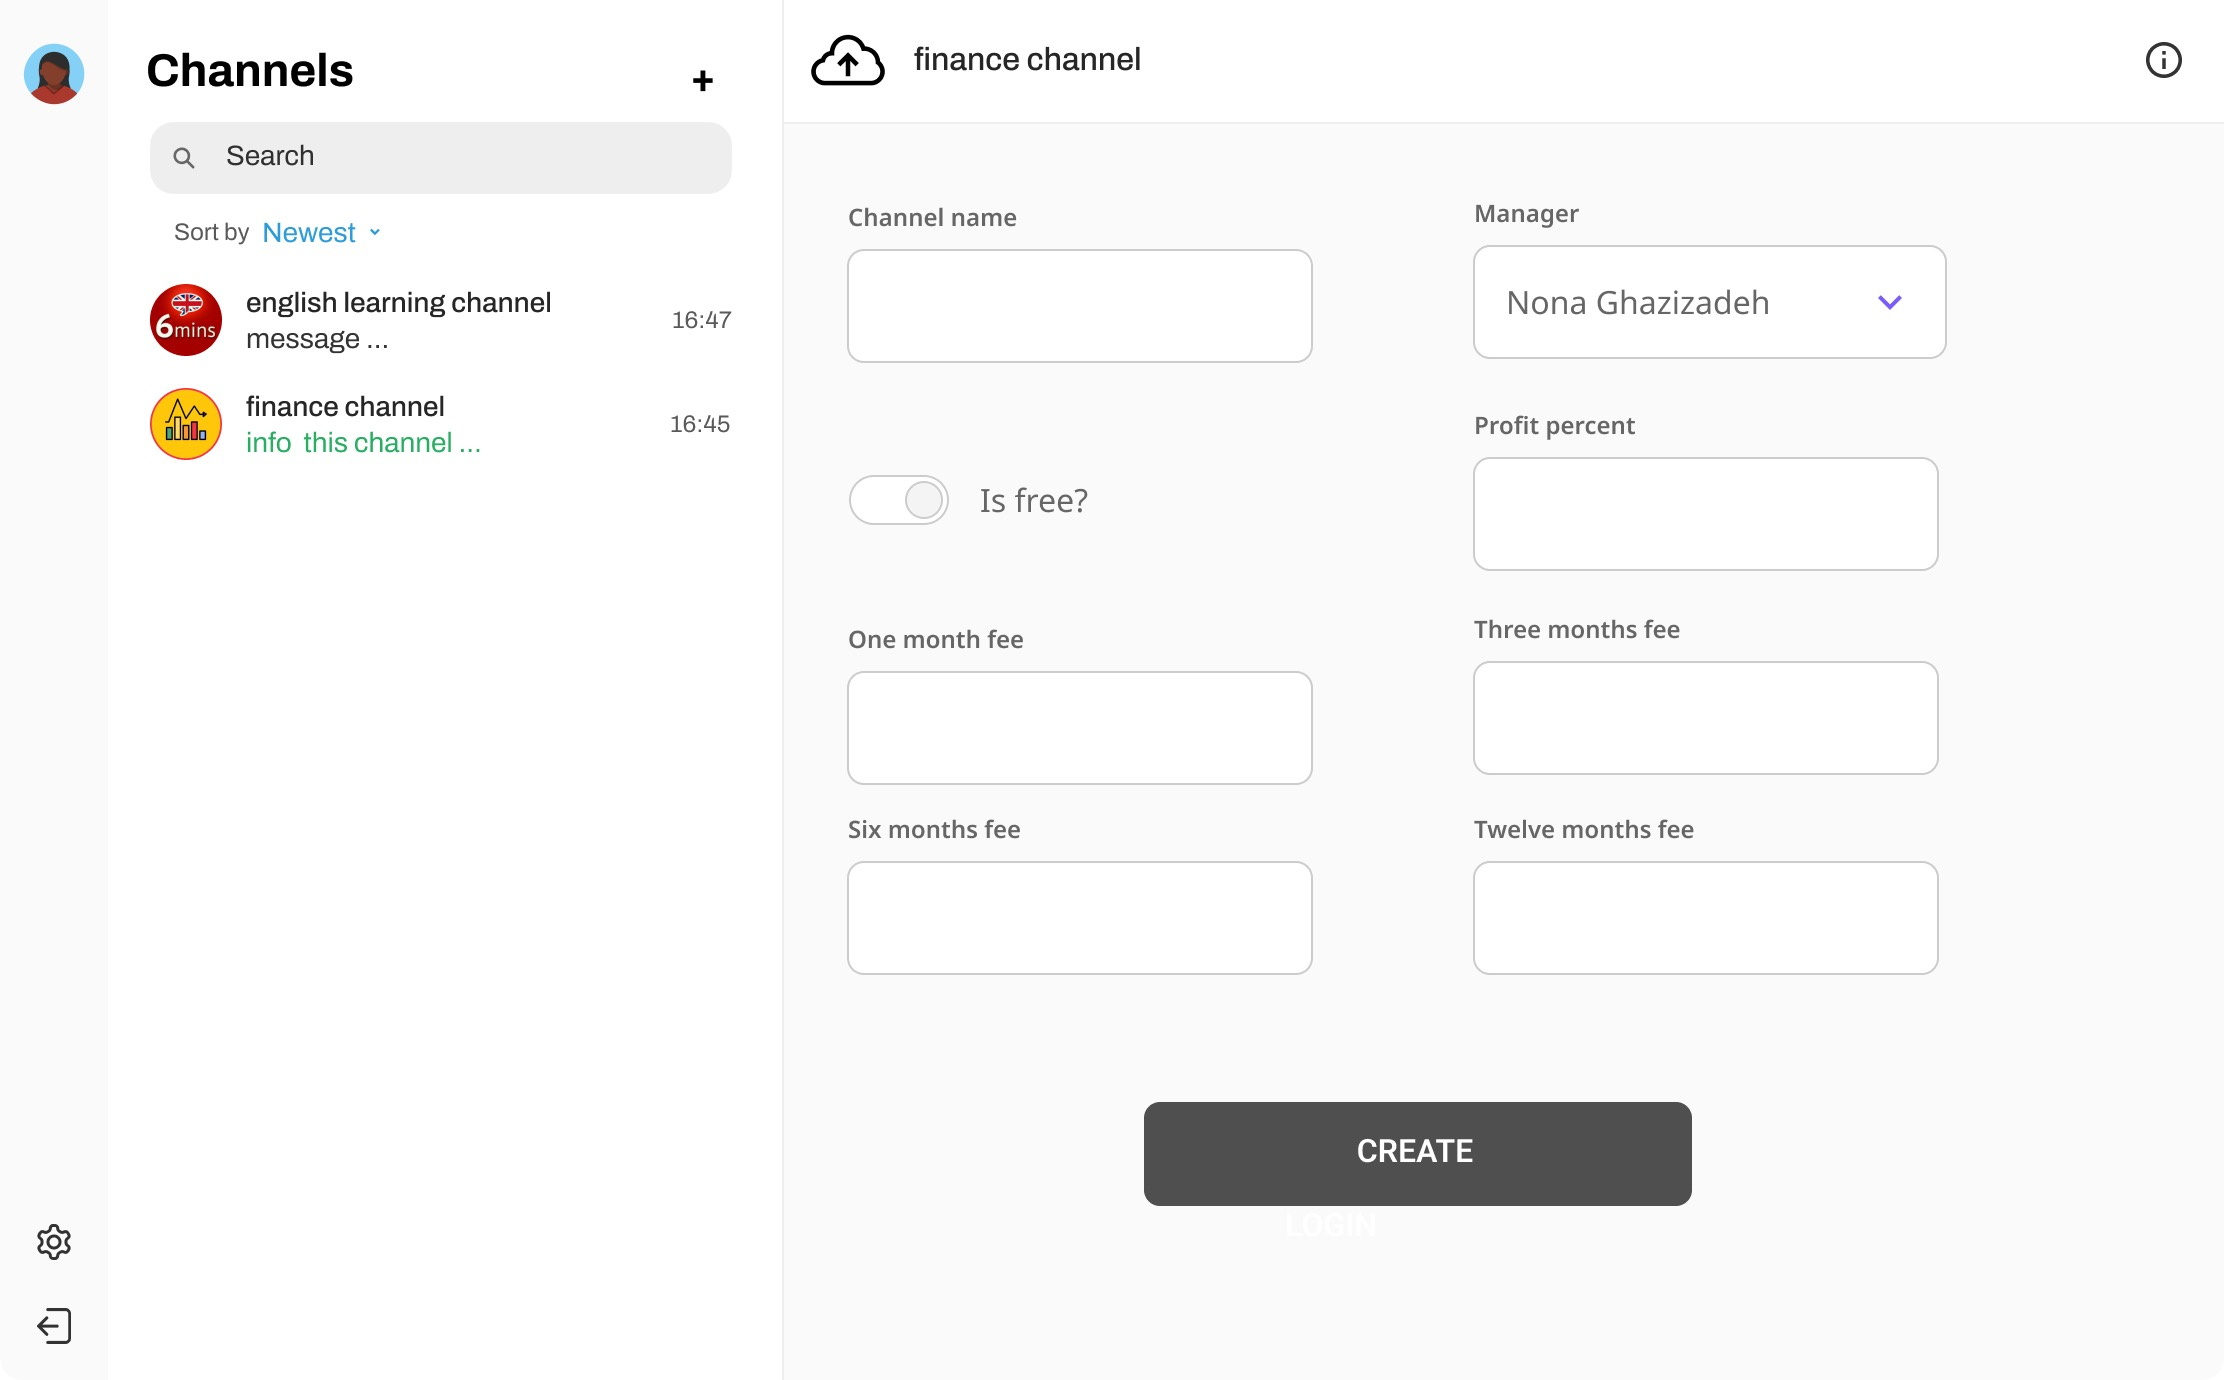
\includegraphics[scale=0.2]{figs/add_channel.jpeg}
‫\شرح{صفحه ساخت کانال}
‫\برچسب{شکل:صفحه ساخت کانال}
‫\پایان{شکل}
